%% amssamp1.tex is nearly identical to amssamp2.tex, except
%% that amssamp2.tex uses the [twocol] option to produce
%% two-column text.

\documentclass{ametsoc}

%\documentclass[twocol]{ametsoc}

%%%%%%%%%%%%%%%%%%%%%%%%%%%%%%%%
%%% To be entered only if twocol option is used

\journal{jcli}

%  Please choose a journal abbreviation to use above from the following list:
% 
%   jamc     (Journal of Applied Meteorology and Climatology)
%   jtech     (Journal of Atmospheric and Oceanic Technology)
%   jhm      (Journal of Hydrometeorology)
%   jpo     (Journal of Physical Oceanography)
%   jas      (Journal of Atmospheric Sciences)	
%   jcli      (Journal of Climate)
%   mwr      (Monthly Weather Review)
%   wcas      (Weather, Climate, and Society)
%   waf       (Weather and Forecasting)
%   bams (Bulletin of the American Meteorological Society)
%   ei    (Earth Interactions)

%%%%%%%%%%%%%%%%%%%%%%%%%%%%%%%%
%Citations should be of the form ``author year''  not ``author, year''
\bibpunct{(}{)}{;}{a}{}{,}

%%%%%%%%%%%%%%%%%%%%%%%%%%%%%%%%

\title{Dominant Anomaly Patterns in the Near-Surface 
Baroclinicity and Accompanying
Anomalies in the Atmosphere and Oceans. 
Part II: North Pacific Basin}

\authors{Mototaka Nakamura\correspondingauthor{Mototaka Nakamura, Japan
Agency for Marine-Earth Science and Technology, 3173-25
Showa-machi, Kanazawa-ku, Yokohama, Kanagawa 236-0001,
Japan.} and Shozo Yamane\thanks{Current affiliation: 
Science and Engineering, Doshisha University, Kyotanabe, Kyoto, Japan.}}

\affiliation{Japan Agency for Marine-Earth Science and Technology, Yokohama,
Kanagawa, Japan} 

\email{moto@jamstec.go.jp}

%\extraauthor{Extra Author}
%\extraaffil{Affiliation, City, State/Province, Country}



\abstract{Variability in the monthly-mean flow and storm track in the North
Pacific basin is examined with a focus on the near-surface baroclinicity.
Dominant patterns of anomalous near-surface baroclinicity found from
EOF analyses generally show mixed patterns of
shift and changes in the strength of near-surface baroclinicity. Composited
anomalies in the monthly-mean wind at various pressure levels based on the
signals in the EOFs show accompanying anomalies in the mean flow up to 50 hPa
in the winter and up to 100 hPa in other seasons. Anomalous eddy fields
accompanying the anomalous near-surface baroclinicity patterns exhibit,
broadly speaking, structures anticipated from simple linear theories of
baroclinic instability, and suggest a tendency for anomalous wave fluxes to
accelerate--decelerate the surface westerly accordingly. However, the
relationship between anomalous eddy fields and anomalous near-surface
baroclinicity in the midwinter is not consistent with the simple linear
baroclinic instability theories. Composited anomalous SST accompanying 
anomalous near-surface baroclinicity often exhibits
moderate values and large spatial scales in the basin, rather than large
values concentrated near the oceanic fronts. In the midsummer and in some
cases in cold months, however, large SST anomalies are found around the
Kuroshio--Oyashio Extensions. Accompanying anomalies in the net surface
heat flux, SST in the preceding and following months, and meridional eddy
heat flux in the lower troposphere suggest active roles played by the ocean
in generating the concomitant anomalous large-scale atmospheric state in some
of these cases.}

\begin{document}

\maketitle


\section{Introduction}

It has now become our basic
knowledge that the extratropical
atmosphere is driven strongly by the horizontal
potential temperature gradient that arises from the
differential solar heating (e.g., Lorenz 1955). The horizontal
gradient in the potential temperature, often referred
to as baroclinicity, is a measure of upper-level wind
steering via thermal wind and a measure of baroclinic
instability in the atmosphere. Baroclinicity in the lower
atmosphere in classic theories of atmospheric stability is
measured by a combination of the static stability and
horizontal temperature gradient, the latter of which is
equivalent to vertical shear in the horizontal wind through
the thermal wind balance (Charney 1947; Eady 1949). In
its original form, the Eady's maximum growth rate for
baroclinic instability $B_{GRMax}$ is defined by $B_{GRMax} =
0.31(|f|/N)(\partial U/\partial_z)$ in a zonally homogeneous steady
mean state, where $U$ is the mean zonal flow, $f$ is the
Coriolis parameter, and $N$ is the Brunt--V\"ais\"al\"a frequency.
Charney's formula is slightly different from the Eady's,
but still incorporates the same effects.


Lindzen and Farrell (1980) first applied the Eady's parameter
to atmospheric data to successfully estimate the
maximum growth rate of baroclinic instability in the troposphere.
Hoskins and Valdes (1990) used its localized
version (i.e., $U$, $N$, and $f$ are all local Eulerian mean values)
as the central parameter in their study of the Northern
Hemispheric storm tracks. This local version, or its simplified
version, has been used successfully as an indicator
of baroclinic wave generation in diagnostic studies of
stormtracks in recent years as well (Nakamura and Sampe
2002; Nakamura and Shimpo 2004; Nakamura et al. 2004).
In our study, the North Atlantic part of which was reported
in Nakamura and Yamane (2009, hereafter Part I), we
define the near-surface baroclinic vector, $\mathbf{B}=B^x\mathbf{i} + 
B^y\mathbf{j}$,
where $B^x= -(g/\theta N)(\partial\theta/\partial y)$ 
and $B^y = (g/\theta N)(\partial\theta/\partial x)$  with
$\theta$ being the monthly-mean potential temperature at 2 m
above the surface, and use it as the central quantity of the
diagnoses. Unless stated otherwise, ``anomalies'' refer to
deviations from the climatology hereafter. Though its meridional
component does not appear in any classic theory of
baroclinic instability, a theory that does incorporate the
effect of $B^y$ shows its important role in enhancing baroclinic
wave generation locally to the east of the mean trough
(Niehaus 1980). In the North Atlantic storm track region,
we indeed found that the substantial zonal gradient in the
surface temperature in and around the Labrador Sea plays
a major role in the large-scale atmospheric state.

\section{The sea surface temperature}
The sea surface temperature
 (SST) is an important factor
in determining $\mathbf{B}$ in the storm-track regions (e.g.,
Hoskins and Valdes 1990; Nakamura et al. 2004; Part I).
SST anomalies (SSTAs) around an oceanic front along the
Gulf Stream (GS), Kuroshio Extension (KE), or Oyashio
Extension (OE) can have a profound impact on $\mathbf{B}$ along
the storm tracks. 

\subsection{A subtle point}
A subtle but important point that has to
be considered carefully in this regard is the spatial scale
and the location of SSTAs with respect to the climatology,
since it is the anomalous surface temperature
gradient whose structure has a spatial scale of the atmospheric
Rossby deformation radius that can exert significant
influence on the large-scale atmospheric flow. 

\subsubsection{Changes in the temperature}
The
high sensitivity of $\mathbf{B}$ to changes in the temperature contrast
across the front and changes in the width of the front, and
the uncertainty in the impact of SSTAs of small spatial
scales on $\mathbf{B}$ make it difficult to assess the effective B
anomalies that are attributable to the SSTAs from the
available data. Moreover, it is uncertain exactly how the
SSTAs in the presence or absence of the land surface
temperature anomalies may or may not produce $\mathbf{B}$ anomalies
that are significant to the atmosphere. 

\paragraph{Complicating factor}The complicating
factor introduced by the land surface must be taken
into account when studying potential roles of extratropical
SSTAs in the extratropical atmospheric anomalies.

Lau (1988) investigated patterns of anomalous storm
track activity and associated low-frequency flow anomalies
by computing empirical orthogonal functions (EOFs)
for high-frequency 500-hPa geopotential height for the
Northern Hemisphere winters. He found that both North
Atlantic and North Pacific storm tracks have a pattern of
meridional shift and a pattern of increased or decreased
eddy activity in the first two EOFs.He also found that these
changes in the storm tracks have symbiotic relationships
with the background flows and have substantial impacts on
the mean flow. Part I approached the issue of the stormtrack
and low-frequency flow variability in connection with
SSTAs in the extratropics, focusing on $\mathbf{B}$ as the key parameter
of diagnoses, and found similar patterns of variability
in the eddy activity and low-frequency flow in the
North Atlantic basin. Much of this variability was connected
to SSTAs in the vicinity of the Gulf Stream in cold
months (Part I). Since the winter North Pacific basin has a
storm track andmean flow that appear to be related to the
oceanic fronts, Kuroshio--Oyashio Extensions (KOE) in
this case, in a manner essentially the same as those in the
North Atlantic basin related to the GS,we have attempted
to find similar results for the North Pacific basin. In this
regard, we have chosen not to project our results onto the
major mode of variability in the extratropical North Pacific
basin, the North Pacific decadal variability (PDV), so
that our presentation and discussion are mostly confined
to the wave--mean flow dynamics of monthly time scale or
shorter.


Our approach to the search for a link between anomalies
in the KOE and the overlying atmosphere is as follows:
(i) identify dominant patterns in anomalous $\mathbf{B}$ in the
storm track for each calendarmonth and identify years in
which the anomaly fits the pattern well, (ii) composite
anomalies in the monthly-mean circulation and highfrequency
transients in the atmosphere to obtain a typical
atmospheric state that accompanies the patterns of
anomalous $\mathbf B$, (iii) composite SSTA to obtain a typical
oceanic state that accompanies and precedes the patterns
of anomalous $\mathbf B$, and (iv) composite anomalous net surface
heat flux that accompanies and precedes the pattern of
anomalous $\mathbf B$. With this approach, we obtain typical pictures
of anomalous states in the atmosphere and oceans
with anomalous $\mathbf{B}$ as their connecting interface.
Section 2 describes the data and procedure to compute
$\mathbf B$. Section 3 describes the climatology and variance of $\mathbf B$.
Dominant patterns of $\mathbf B$ are shown in section 4, followed by
composited anomalies in various atmospheric fields and
SST in section 5. Finally, we present our discussion on the
results, examining a potential cause--effect relationship
between anomalies in the SST and atmosphere in section 6.


Figure \ref{fig1} shows the climatology of $Bx$, $U^{200}$,
$\overline{V'\theta'}^{850}$, $\overline{V'\theta'}^{200}$, 
$MR^{z850}$, $U^{1000}$, SST, and $F_h$ for February and
August as examples of the reference state in the winter
and summer. The numeric superscript indicates the pressure
level in hPa. The seasonal mean is visibly more
diffused in structure, particularly for Bx, than those
shown in Fig.~\ref{fig1}. There are no surprises in the overall
picture of Bx. The regions of large land--sea temperature
contrast and the oceanic fronts show very large Bx in cold
months. The position of Bx maximum in the storm track
region is found along theKOEregion throughout the year.
The zonally elongated band of large Bx in the storm track
is generally wider in cold months than in warm months.
In fact, large Bx values that presumably accompany the
Kuroshio and its extension in the cold months vanish in
the summer (Figs. 1a,b). The seasonal variation in the Bx
values in the storm track basically follows that of the
north--south differential heating--largest in the winter and
smallest in the summer. As reported by Nakamura et al.
(2004), the $U^{200}$ maximum is displaced southward from the
Bx maximum visibly in winter months (Fig.~1a), although
U200 is generally large over the area of large Bx in the core
of the storm track. The southward displacement of the
U200 maximum from the Bx maximum in the storm track
is less pronounced or even reversed in warmer months
(Fig.~1b). We note that the structure of the climatological
Bx generally reflects those of ($\partial{\theta^{2{\textrm m}}}/\partial{y}$) with some exceptions where
the surface slope contributes significantly to Bx
in isolated areas over the land, most notably around the
Himalayas.

The position and structure of the storm track as indicated
by $\overline{V'\theta'}^{850}$
and $\overline{V'V'}^{200}$
are, at least for the winter,
essentially the same as those reported in earlier studies on
the storm tracks (e.g., Chang et al. 2002). The maxima in
$\overline{V'\theta'}^{850}$
and $\overline{V'V'}^{200}$ are located in the band of large Bx.


\section{Data and calculation procedures}
The data used to calculate $\mathbf{B}$ are the monthly-mean
temperature at 2 m above the surface ($T^{2m}$) and temperature
at pressure levels available from the 40-yr European
Centre for Medium-Range Weather Forecasts (ECMWF)
Re-Analysis (ERA-40; Uppala et al.~2005). We chose
the ERA-40 $T^{2m}$ data rather than the National Centers
for Environmental Prediction--National Center for Atmospheric
Research (NCEP--NCAR) reanalysis products
for its explicit inclusion of the observed near-surface temperature
in producing the $T^{2m}$ data. The monthly-mean
surface pressure data from the NCEP--NCAR reanalyses
(Kalnay et al. 1996) were used to determine the pressure
levels to be used for $\mathbf B$ calculation, and to calculate $\theta$ 
at 2 m
above the surface from $T^{2m}$. We used the NCEP--NCAR
surface pressure data for convenience, since we had already
compiled the dataset for calculating transient eddy
fluxes to be mentioned later and the ERA-40 surface
pressure data are not readily available. We later compared
the NCEP--NCAR monthly-mean sea level pressure with
that of ERA-40, and found the difference between the two
products to be immaterial for the purpose of the current
study. We also used ERA-40 monthly-mean horizontal
wind and geopotential height at pressure levels, net surface
heat flux, Fh (the sum of latent heat flux, sensible heat flux,
solar radiation, and the thermal radiation), and Hadley
Centre sea surface temperature data (Rayner et al. 2003)
to compile anomaly composites accompanying anomalous
patterns in $\mathbf B$. In addition, we used 6-hourly temperature
and wind data from the NCEP--NCAR reanalyses to
compute various eddy fields. The accuracy of the Fh data
used here is, as true for other reanalyses surface heat flux
products, may not be so high to produce reliable anomaly
composites.


We computed $\mathbf{B}$ near the surface by calculating the
horizontal gradient in $\theta^{2{\textrm m}}$, using the centered finite differencing,
and calculating $N$ from the lowest three vertical
pressure levels that are location dependent because of
topography. Both $\nabla\theta^{2{\textrm m}}$ and $N$ were calculated locally as in
Hoskins and Valdes (1990) and Nakamura and Shimpo
(2004). The entire 45 yr from September 1957 to August
2002 were used for the Northern Hemisphere. To resolve
the dominant modes in $\mathbf{B}$ arising from the land--sea temperature
contrast, one may need much higher horizontal
resolution in the data. The relatively coarse horizontal
resolution of the data may artificially suppress the significance
of the variability associated with the land--sea temperature
contrast.One should keep this limitation in mind.
The 6-hourly bandpassed (period of 2--7 days) eddy
fields and ultra-low-frequency (period of 30 days and longer)
background fields were computed from the NCEP--
NCAR reanalyses, using simple time filters (Lau and Lau
1984) first. The filtered time series were then visually examined
against the raw time series and, then, used to calculate
the slowly evolving bandpassed meridional velocity
variance ($\overline{V'V'}$), meridional temperature flux ($\overline{V'\theta'}$), and
the three-dimensional transient wave activity flux defined
on a zonally varying basic state by Plumb (1986). The wave
activity flux consists of the zonal and meridional advective
fluxes (MU and MV), the zonal and meridional
radiative fluxes (MRx and MRy), and the radiative vertical
flux (MRz). The flux is essentially the Eliassen--Palm
flux (Eliassen and Palm 1961) in a zonally inhomogeneous
mean flow (Plumb 1986). The wave activity flux was calculated
from February 1948 to November 2004 only for
the extratropics poleward of 208 latitude. Also, it was
calculated only from 850 to 30 hPa because of the double
differentiation with respect to pressure required for the
calculation. The flux of particular interest in this study is
the vertical component. Here MR$^z$ is defined by
\[
MR^z=
\frac{
pf \cos\phi}
{p^0|\nabla h\bar q|(d\theta_0/dz)}
\left(\frac{\partial\bar q}{\partial x}
\overline{U'\theta'} +
\frac{\partial\bar q}{\partial y}
\overline{V'\theta'}\right), 
\]
where $q$ is quasigeostrophic potential vorticity, $p$ is the
pressure, $p^0$ is the reference surface pressure set to
1000 hPa here, $\theta_0$ is the area-weighted ultra-low-frequency
hemispheric mean potential temperature at each height,
u9 is the bandpassed potential temperature, and z is the
geopotential height. An overbar denotes an ultra-low frequency
component and a prime denotes bandpassed
component. The 6-hourly time series of wave fluxes was
computed by using the time series of ultra-low-frequency
fields as the basic-state and high-frequency fields as eddies.
In short, the time series was calculated by changing the
meaning of an overbar from the time mean state to an
ultra-low-frequency state, and changing the meaning of a
prime from a departure from the mean to a high-frequency
state. The 6-hourly eddy time series was averaged over each
month to produce monthly-mean time series. This dataset
allows us to examine anomalous eddy fields accompanying
anomalous $\mathbf B$ in specific months. The climatology for
the eddy fields was computed from 46 yr, January 1958 to
December 2003. The calculation of the wave activity and
its flux is described in detail by Nakamura et al. (2010).


\section{Climatology and variance}
The climatology and variance of $Bx$ and $By$ were computed
for each calendar month and examined closely for
their spatial and temporal structures. The monthly climatology,
rather than the seasonal climatology, is used as the
reference in our study, to avoid contamination of the diagnostic
results arising from differences in the climatology
between two successive months. Unlike in the North Atlantic
basin reported in Part I, we found the impact of $By$
variations on the large-scale atmospheric state in the
North Pacific basin much weaker than that of Bx variations,
presumably because of themore zonal orientation of
the KOE in comparison to the Gulf Stream and North
Atlantic Current. In the following, thus, we focus our
presentation on the climatology and variations of $Bx$ and
their impact on the large-scale atmospheric state.

Sample citations: \citet{Becker+Schmitz2003}, \citet{Knutti2008},
and \citep{MeixnerEA2002,Kuji_Nakajima2002,EmeryEA1986}.

%%%%%%%%%%%%%%%%%
%ACKNOWLEDGMENTS
%%%%%%%%%%%%%%%%%

\acknowledgments
We thank two anonymous reviewers for their comments, which helped
to improve the manuscript.

%%%%%%%%%%%%%%%%%
%APPENDIXES
%%%%%%%%%%%%%%%%%
\appendix
\appendixtitle{Appendix Title}

\subsection*{Appendix section head}

Here is a sample appendix.
\begin{equation}
\frac{
pf \cos\phi}
{p^0|\nabla h\bar q|(d\theta_0/dz)}
\end{equation}

\appendix[B]
\appendixtitle{Second Appendix Title}
\subsection{Sample appendix section head}
Second appendix example.
\subsection{Sample appendix section head}
\begin{equation}
\left(\frac{\partial\bar q}{\partial x}
\overline{U'\theta'} +
\frac{\partial\bar q}{\partial y}
\overline{V'\theta'}\right) 
\end{equation}


%%%%%%%%%%%%%%%%%
%REFERENCES
%%%%%%%%%%%%%%%%%

\bibliographystyle{ametsoc2014}
\bibliography{references}

%%%%%%%%%%%%%%%%%
% TABLES
%%%%%%%%%%%%%%%%%

\begin{table}
\caption{Percentage of variance explained by the first four
EOFs for the North Pacific Bx. The degree of separation between
EOF1 and EOF2 and EOF2 and EOF3, based on the North et al.
(1982) criterion, is indicated by good (GD) and not good or marginal
(NG).}
\begin{tabular*}{\hsize}{@{\extracolsep\fill}lcccccc@{}}
\topline
Month& EOF1& Split &EOF2& Split& EOF3& EOF4\\
\midline
\ Jan& 29& NG& 24& GD& 10& 5\\
\ Feb& 39& GD& 20& GD& \phantom{1}7 &6\\
\ Mar& 31& GD& 14& NG& 10& 6\\
\ Apr& 23& GD& 14& NG& 10& 7\\
\ May& 19& GD& 12& NG& 10& 7\\
\ Jun& 19& GD& 12& NG& 10& 9\\
\ Jul& 18& NG &13& NG& \phantom{1}9& 7\\
\ Aug& 18& NG& 13& NG& 11& 9\\
\ Sep &17& NG& 13& NG& 10& 8\\
\ Oct &16& NG& 13& GD& \phantom{1}8& 7\\
\ Nov &19 &NG& 16& NG& 11& 8\\
\ Dec& 33& GD& 18& GD& 10& 6\\
\botline
\end{tabular*}
\end{table}



\begin{table}
\centering
\caption{Years selected for anomaly composites for the positive
phase of $B^x$ EOF1.}
\begin{tabular}{lc}
\topline
Month& Yr of positive phase\\
\midline
\ \ Jan& 1961, 1969, 1978, 1979, 1988, 1990, 1992, 1994\\
\ \ Feb& 1964, 1977, 1978, 1980, 1983, 1986, 1988, 2000, 2001\\
\ \ Mar& 1970, 1973, 1979, 1980, 1984, 1988, 2000\\
\ \ Apr& 1959, 1961, 1962, 1963, 1968, 1972, 1983, 2002\\
\ \ May& 1971, 1984, 1993, 1996, 2000\\
\ \ Jun& 1981, 1983, 1984, 1993, 1998\\
\ \ Jul& 1961, 1972, 1973, 1978, 1994, 2000\\
\ \ Aug& 1967, 1970, 1973, 1978, 1994, 1999\\
\ \ Sep& 1975, 1977, 1988, 1989, 1994, 1998, 1999\\
\ \ Oct& 1962, 1977, 1998, 1999, 2001\\
\ \ Nov& 1985, 1986, 1987, 1988, 1991, 1998\\
\ \ Dec& 1957, 1968, 1972, 1978, 1979, 1990\\
\botline
\end{tabular}
\end{table}

\begin{table}
\centering
\caption{Years selected for anomaly composites for the negative
phase of $B^x$ EOF1.}
\begin{tabular}{lc}
\topline
Month& Yr of negative phase\\
\midline
\ \ Jan&1962, 1963, 1968, 1974, 1991, 1996, 1997\\
\ \ Feb& 1959, 1963, 1971, 1974, 1976, 1979, 1985, 1989, 1990, 1994\\
\ \ Mar& 1963, 1968, 1972\\
\ \ Apr& 1984, 1988, 1993, 1996, 1999, 2000\\
\ \ May& 1961, 1963, 1983, 1987, 1997\\
\ \ Jun& 1961, 1972, 1978, 1980, 1982, 1986\\
\ \ Jul& 1964, 1974, 1980, 1983, 1986, 1988, 1993\\
\ \ Aug& 1980, 1987, 1991, 1993, 1997\\
\ \ Sep& 1959, 1963, 1969, 1983, 1985, 1993\\
\ \ Oct& 1957, 1986, 1993, 1996, 1997\\
\ \ Nov& 1958, 1968, 1970, 1982, 1997\\
\ \ Dec& 1969, 1974, 1976, 1985, 1998, 1999, 2000, 2001\\
\botline
\end{tabular}
\end{table}

%%%%%%%%%%%%%%%%%
% FIGURES
%%%%%%%%%%%%%%%%%

\begin{figure}[t]
\centerline{\includegraphics[width=\textwidth]{figone.pdf}}

\caption{Climatology of $Bx (10^{-6} s^{-1}$, color) and $U^{200}$(m s$^-1$,
contours) for (a) February and (b) August; $\overline{V'\theta'}^{850}$
(K m s$^-1$, color) and 
$\overline{V'V'}^{200}$
(m$^2$ s$^{-1}$, contours) for (c) February and (d) August; MR$^{z850}$ 
(10$^{-3}$ m$^2$ s$-2$, color) and $U^{1000}$ (m s$^{-1}$, contours) 
for (e) February and (f) August;
and SST (K, color) and $F_h$ [10$^5$ J m$^{-2}$ (6 h)$^{-1}$] for (g)
February and (h) August. Red rectangles indicate the domain of EOF
calculations.} \label{fig1} 
\end{figure}

\begin{figure}[p]
\centerline{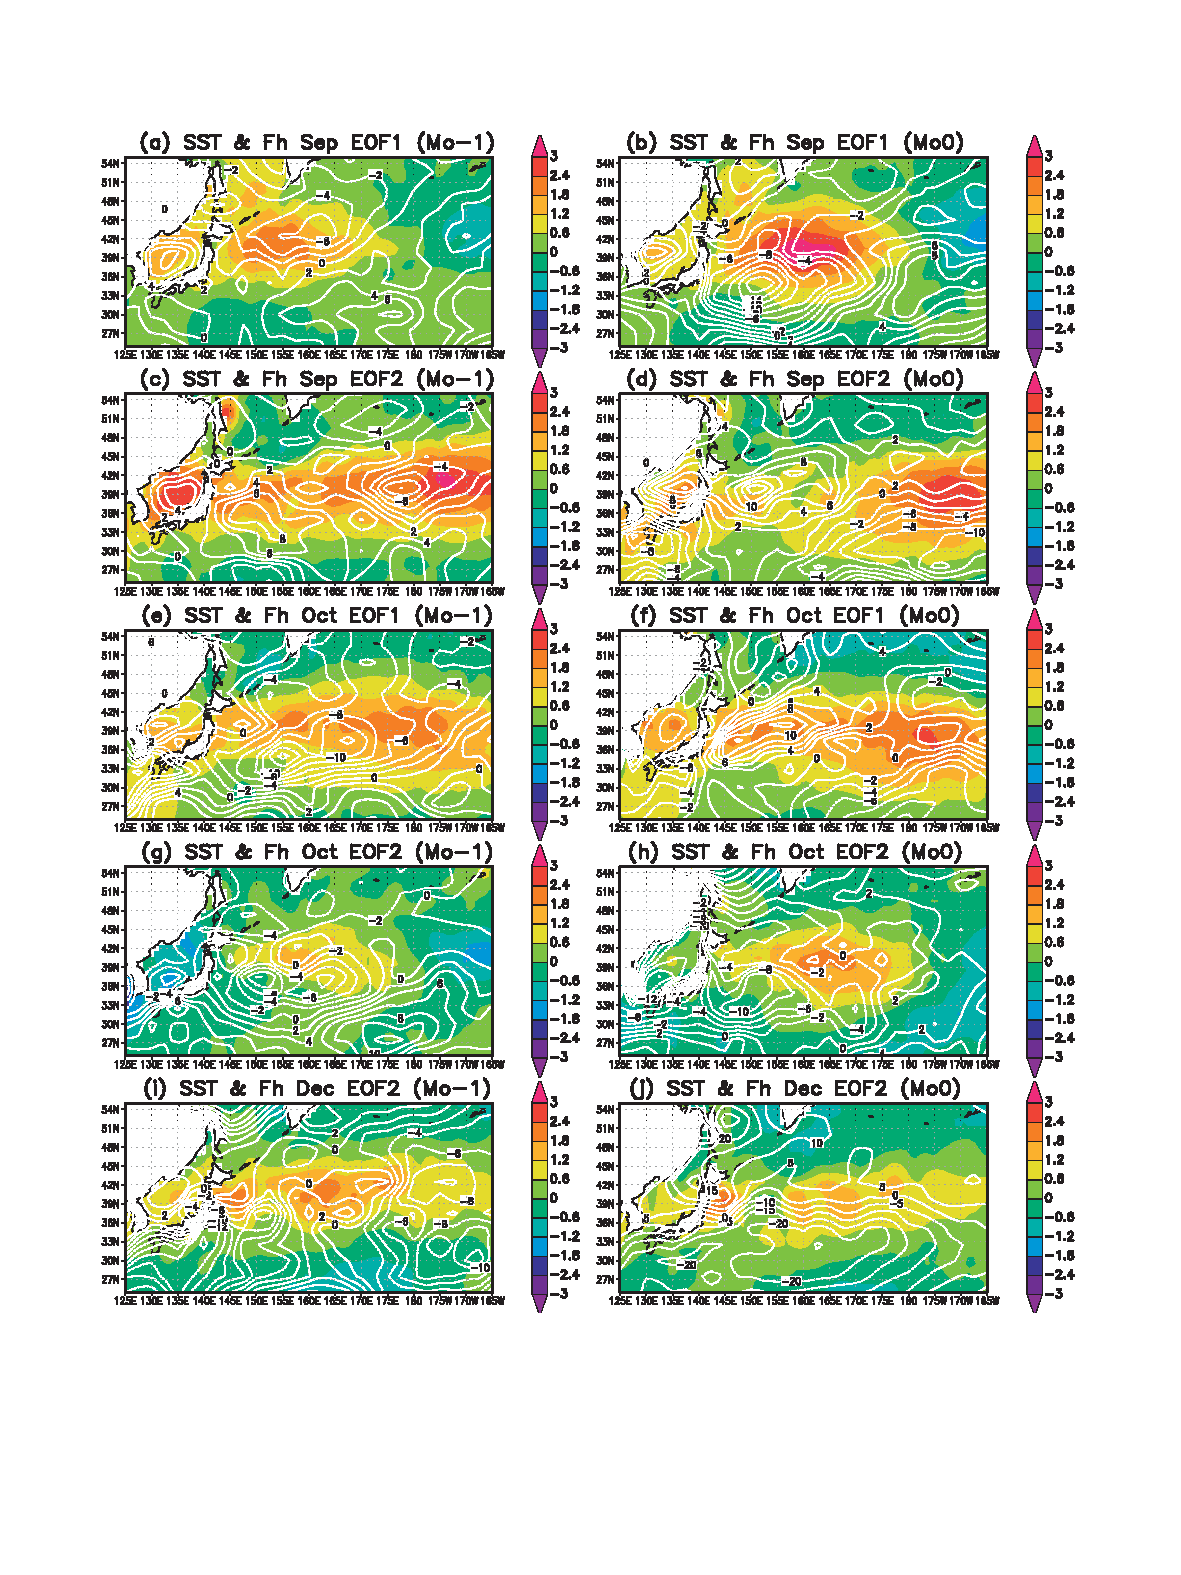
\includegraphics{FigTwo.pdf}}
\caption{As in Fig.~10, but for (a),(b) September EOF1; (c),(d) September EOF2; (e),(f) October EOF1; (g),(h) October EOF2; and
(i),(j) December EOF2.}
\end{figure}

\begin{figure}
 \centerline{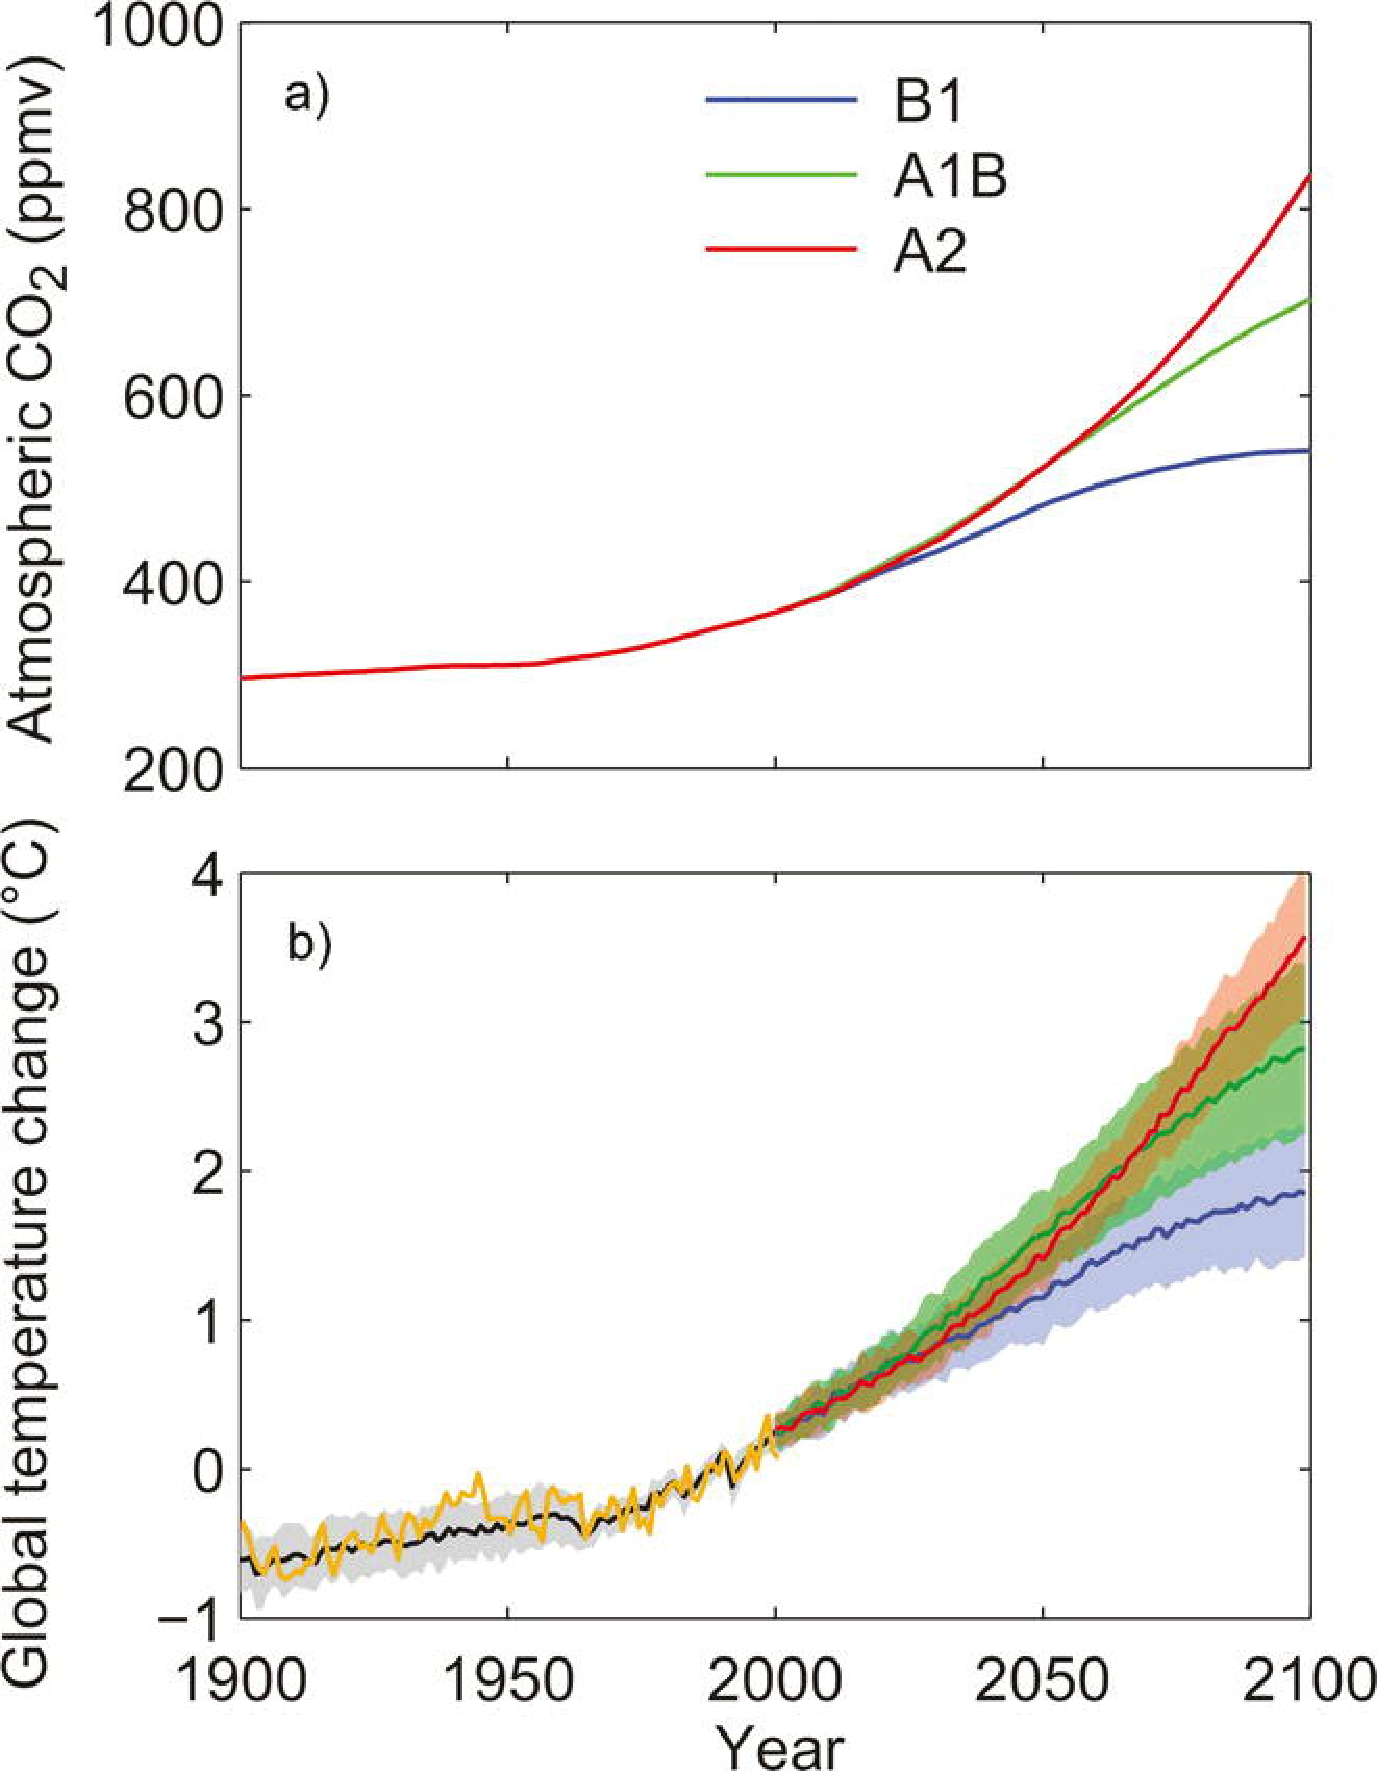
\includegraphics[width=19pc]{figure01.pdf}}
\appendcaption{A1}{Here is an appendix, single column figure caption.}
\end{figure}




\end{document}





